\section{Algorithms and Implementation}
In this section, we describe the filtering algorithms we used: fixed size grid filter, tree-based dynamic grid filter, particle filter, filter based on a polynomial of fixed degree, and a filter based on feed-forward deep neural networks. We implemented the algorithms in C++, the simulation data was generated using Octave (Matlab). The source code is available at \textit{https://github.com/AbheekG/filter}. We used the Eigen library and some code from \textit{https://github.com/yixuan/MiniDNN/} to implement the feed-forward neural network. For running in Nao, the LARG codebase given to the class was used.

The \textit{Filter} C++ class contains the parameters and functions common to all filtering algorithms, like sensor and motion measurement functions, timing functions, I/O, etc. Each individual algorithm has its own derived class.

\subsection{Particle Filter}
It is similar to what we did in assignment 5 (localization), with slight modifications to fit our testing framework. The class \textit{ParticleFilter} implements this algorithm. The number of particles is given as the hyper-parameter.

\subsection{Fixed Grid Filter}\label{gf_def}
In this method, the entire state space is divided into a grid of a fixed number of points. For each grid point, the value of the belief distribution is stored. The grid structure is pre-decided and doesn't change with the time or the belief distribution.

The algorithm works for any arbitrary dimension and grid size. Each grid is a hyperrectangle, e.g., a rectangle for 2-D. It stores the function values in a linear vector with appropriate indexing for multi-dimension. The class \textit{GridFilter} implements this algorithm. The grid size is given as the hyper-parameter.

\begin{figure}
\caption{Fixed grid filter. (Figure taken from \cite{prob})}
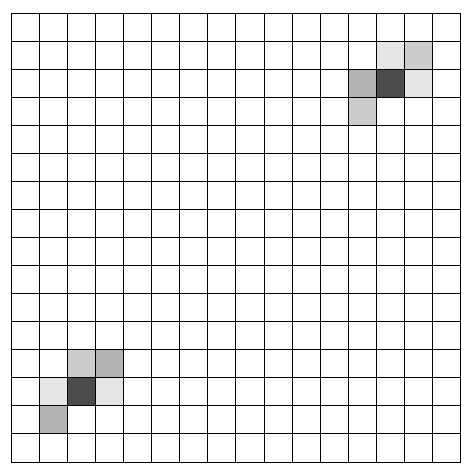
\includegraphics[width=\linewidth]{grid}
\end{figure}

\subsection{Dynamic Grid Filter}
Similar to the fixed grid filter\ref{gf_def}, in this method also the entire domain of the belief distribution is divided into sub-domains (grid block) and the value of the belief distribution is approximated for each grid block.

The entire grid is stored in the form of a tree. Each node corresponds to a grid block. A node of the tree is a leaf node if the total probability (weight) for the grid block (hyperrectangle) corresponding to the node is less than a given probability threshold. If the weight of a node is more than the probability threshold then its grid block is partitioned into its children. For example, the root of the tree has a grid block with the size of the entire domain for the robot state and probability $1$. If the probability threshold is less than $1$ then the root will have children.

The nodes are branched and collapsed dynamically as the belief distribution changes. A node whose weight goes above the threshold is branched, while if it goes below the threshold it is collapsed and its children vanish. We also have a partial implementation for using different lower and upper probability thresholds. The class \textit{DynamicGridFilter} implements this filtering method. The probability thresholds are given as the hyper-parameters.

\begin{figure}
\caption{Dynamic grid filter. (Figure taken from \cite{prob})}
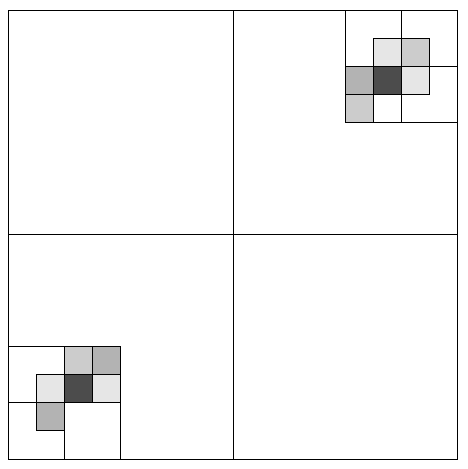
\includegraphics[width=\linewidth]{dgrid}
\end{figure}

\subsection{Polynomial Filter}
In this method, we approximate the belief using a polynomial of fixed degree. The original state is converted to a new modified state with higher order terms, and then the least square fit is done to find the coefficients of the polynomial. The class \textit{PolynomialFilter} implements this algorithm. The degree is given as a hyperparameter. Due to lack of time, we could only have implementation up to degree $2$.

\subsection{Neural Network Filter}
In this method, we use a feed-forward deep neural network (NN). The input to the neural network is a state and output is the value of the belief distribution corresponding to the state. Essentially, the function represented by the NN is the approximate belief distribution. The neural network is partially trained in each time step (sensor and motion update). For each time step, the input data (set of states), $X$, is generated depending on the previous belief (or NN), more samples from areas with higher weight and less from the lower weight. The output data, $y$, is generated as a product of current sensor measurement and previous belief. Currently, the motion is updated by doing a shift in the $X$, assuming that motion updates don't have an error.

The class \textit{NeuralNetwork} implements this algorithm. All the standard hyper-parameters for a neural network, like the number of layers, size of each layer, learning rate, batch size, etc. are applicable here also.